\section{Architecture for Automatic Provisioning of Cloud Services}
\label{related:architecture}

\citeauthor{provisioning:architecture} present an extensible architecture for automatic provisioning of cloud infrastructure and services at different cloud providers.
They define a cloud service as a number of software components, their configuration, and the cloud infrastructure they are running on.
Therefore, to provision a cloud service, one must first provision the cloud infrastructure, then install the software components and finally configure them.
For this process they designed a so called service orchestrator~\autocite{provisioning:architecture}.

\begin{figure}[!htbp]
	\centering
	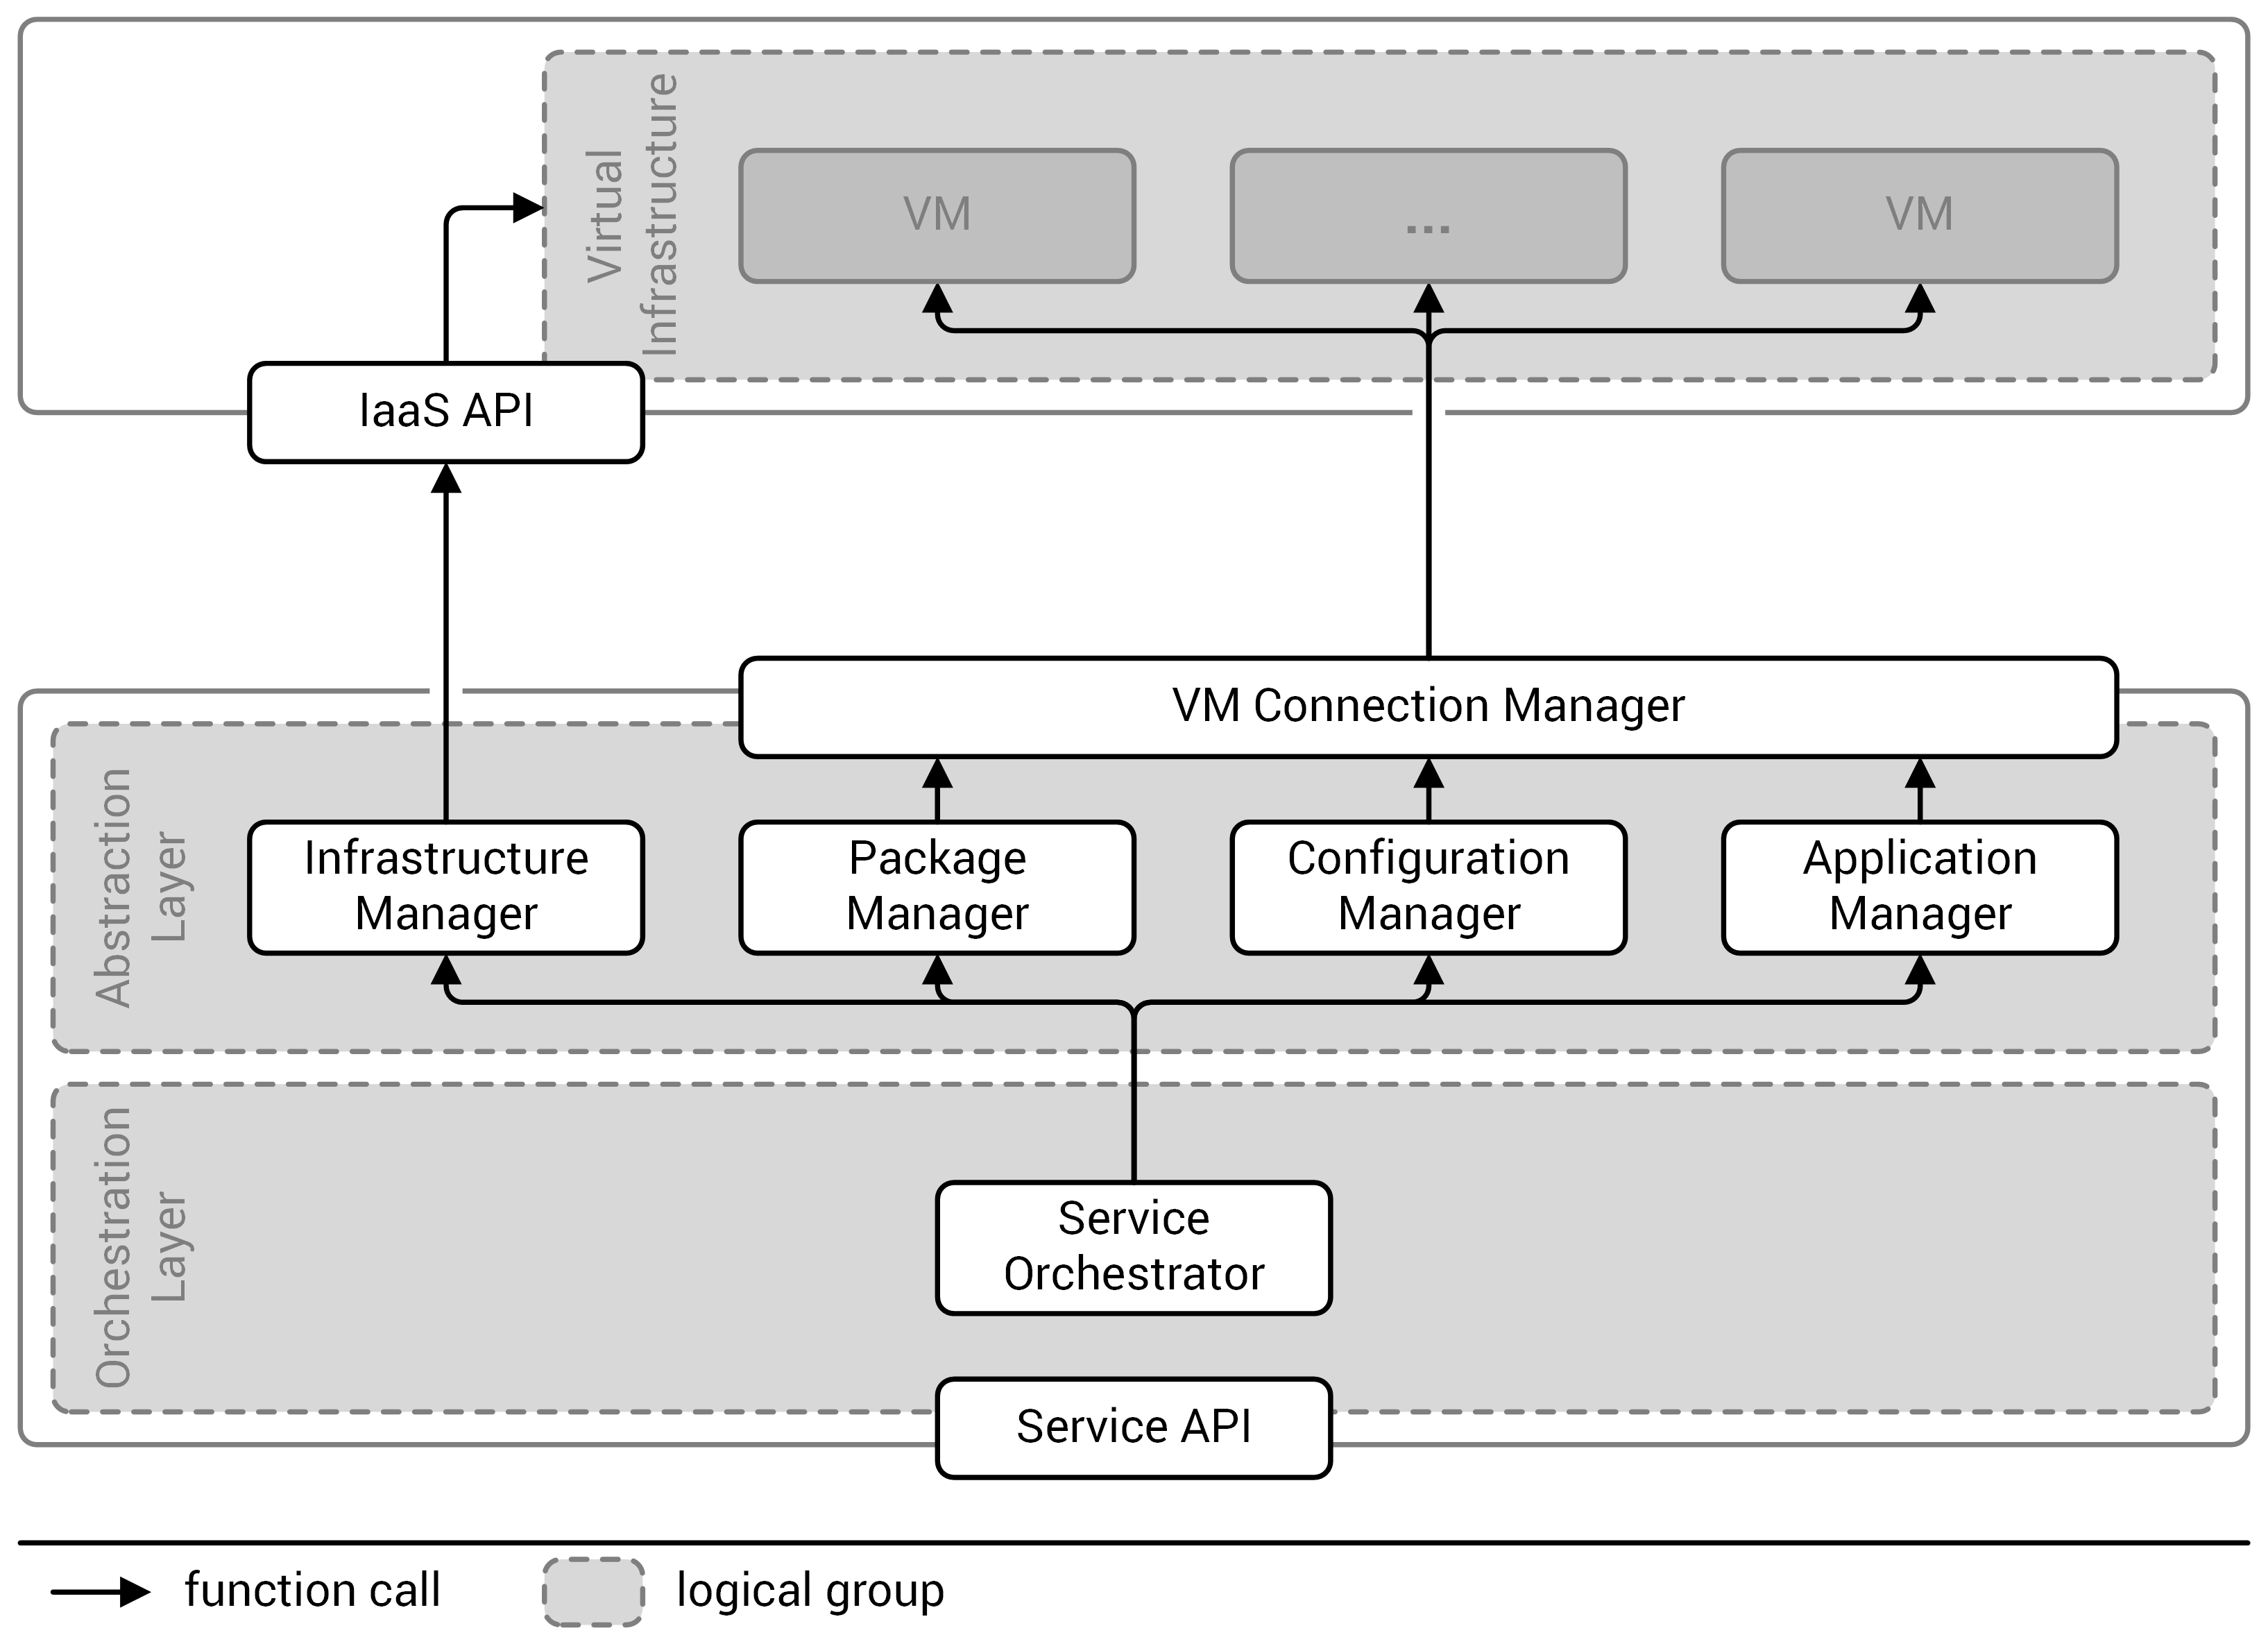
\includegraphics[resolution=600]{related/assets/automatic_architecture}
	\caption{Simplified architecture for automatic provisioning of cloud services~\autocite[based on][]{provisioning:architecture}}
	\label{image:automatic_architecture}
\end{figure}

\autoref{image:automatic_architecture} shows a simplified overview of the service orchestrator architecture.
Users can submit service models via a service API, shown at the bottom of \autoref{image:automatic_architecture}.
The service model describes the topology of a cloud service, the components it consists of and their configuration.
This model is used by the service orchestrator to provision new cloud services and to trigger reconfiguration and topology changes of existing services~\autocite{provisioning:architecture}.

The service orchestrator is build in two layers.
The orchestration layer, shown at the bottom of \autoref{image:automatic_architecture}, picks up the service model and delegates the different steps that are necessary to provision the cloud service to the abstraction layer.
The deployment steps will be executed in parallel wherever dependencies allow it.
The abstraction layer, shown in the middle of \autoref{image:automatic_architecture}, provides abstract methods to handle the management, installation, configuration, and starting of software.
It consists of five different managers for infrastructure, packages, applications, configuration, and VM connections~\autocite{provisioning:architecture}.

The infrastructure manager abstracts away different APIs of cloud providers for provisioning cloud infrastructure.
It is used to create new VMs at a specific cloud provider, shown at the top of \autoref{image:automatic_architecture}.
These can then can be used by the other managers to create the requested cloud service.
The VM connection manager offers a unified interface for different communication methods, for example \nom{Secure Shell}{SSH}, \nom{Remote Desktop Connection}{RDC}, \nom{Virtual Network Computing}{VNC}, and Telnet.
The package, configuration, and application managers use the interface provided by the connection manager to send their commands to the VMs at the cloud provider~\autocite{provisioning:architecture}.

The package manager can install software packages in different environments, for example with existing package managers like \nom{Advanced Packaging Tool}{APT}, or directly on the file system.
The configuration manager offers a unified interface for component specific configuration methods, such as file templates or configuration APIs.
The application manager manages the state of software components, i.e. starting and stopping them.
Together, these managers can install, configure, and manage the requested cloud service on the VMs provided by the cloud provider~\autocite{provisioning:architecture}.
